\section{Models}
\label{sec-emnlp2016:models}

We use the extracted causal tuples to train three distinct distributional similarity models that explicitly capture causality. 

{\flushleft \textbf{Causal Embedding Model (cEmbed):}}
The first distributional similarity model we use is based on the skip-gram word-embedding algorithm of \citet{mikolov2013distributed}, which has been shown to improve a variety of language processing tasks\footnote{Chris Manning recently called embedding models the Sriracha sauce of NLP.} 
including QA~\citep{yih13,fried2015higher}.  In particular, we use the variant implemented by \citet{levy2014dependency} which modifies the original algorithm to use an arbitrary, rather than linear, context. 
Our novel contribution is to make this context task-specific: intuitively, the context of a cause is its effect.  Further, these contexts are generated from tuples that are themselves bootstrapped, which minimizes the amount of supervision necessary.

The Levy and Goldberg model trains using single-word pairs, while our causal mentions (CM) could be composed of multiple words.  
For this reason, we decompose each cause--effect tuple, $(CM_c,CM_e)$, such that each word $w_c \in CM_c$ is paired with each word $w_e \in CM_e$. 

After filtering the extracted cause-effect tuples for stop words and retaining only nouns, verbs, and adjectives, we generated over 3.6M $(w_c, w_e)$ word-pairs\footnote{For all models proposed in this section we used lemmas rather than words.} from the approximately 800K causal tuples.

The model learns two embedding vectors for each word, one for when the word serves as a target word and another for when the word serves as a context word.  Here, since the relation of interest is inherently directional, \textit{both} sets of embeddings are meaningful, and so we make use of both -- the target vectors encode the effects of given causes, whereas the context vectors capture the causes of the corresponding effects.  
As an example, consider the causal relation between the words \textit{wind} and \textit{damage} and the lack of a causal relation between \textit{wind} and \textit{popcorn}.  Given the previously described embeddings, after training we expect that the target (cause) vector for \textit{wind} will be closer to the context (effect) vector for \textit{damage} than to context vector for \textit{popcorn}, indicating a more likely causal relation.

{\flushleft \textbf{Causal Alignment Model (cAlign):}}
Monolingual alignment (or translation) models have been shown to be successful in QA \citep{Berger:00,Echihabi:03,Soricut:06,Riezler:etal:2007,Surdeanu:11,yao2013}, and in Chapter \ref{chapter:naacl2015} we showed that they can be successfully trained with less data than embedding models~\citep[see also][]{sharp-EtAl:2015:NAACL-HLT}. 
% Further, Fried et al.~\citeyear{fried2015higher} demonstrated that \todo{dest. distribution as semantic model of the source concept, which is important for our task as well.} % ms: nice, but no space

To evaluate these observations in this context, we train an alignment model that ``translates'' causes (i.e., the ``source language'') into effects (i.e., the ``destination language''), using our cause--effect tuples. 
This is done using IBM Model 1~\citep{Brown:93} and GIZA++~\citep{och03}. 

\begin{figure}[t!]
\begin{center}
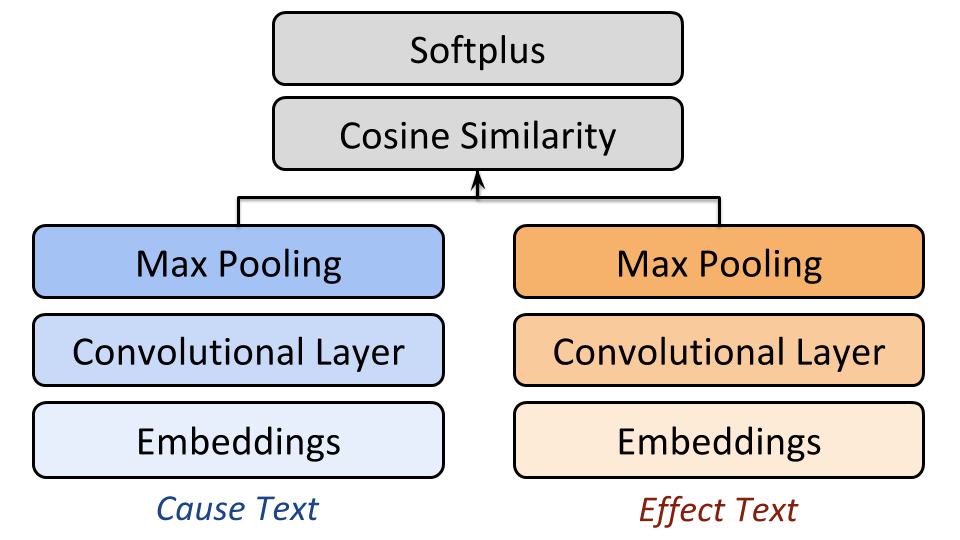
\includegraphics[width=0.7\textwidth]{mainmatter/emnlp2016-causal/cnn2.png}
%space{-2mm}
\caption{{\footnotesize Architecture of the causal convolutional network. }}
%space{-6mm}
\label{fig:cnn}
\end{center}
\end{figure}

{\flushleft \textbf{Causal Convolutional Neural Network Model (cCNN):}}
Each of the previous models have at their root a bag-of-words representation, which is a simplification of the causality task. To address this potential limitation, we additionally trained a convolutional neural network (CNN) which operates over variable-length texts, and maintains distinct embeddings for causes and effects.  The architecture of this approach is shown in Figure~\ref{fig:cnn}, and consists of two sub-networks (one for cause text and one for effect text), each of which begins by converting the corresponding text into 50-dimensional embeddings.  These are then fed to a convolutional layer,\footnote{The convolutional layer was lightly tuned to contain 100 filters, had a filter length of 2 (i.e., capturing bigram information), and an inner ReLU activation.} which is followed by a max-pooling layer of equal length.
Then, these top sub-network layers, which can be thought of as a type of phrasal embedding, are merged by taking their cosine similarity.  Finally, this cosine similarity is normalized by feeding it into a dense layer with a single node which has a softplus activation.  
In designing our CNN, we attempted to minimize architectural and hyperparameter tuning by taking inspiration from \citet{iyyer2015deep}, preferring simpler architectures.
We train the network using a binary cross entropy objective function and the Adam optimizer~\citep{kingma2014adam}, using the Keras library~\citep{chollet2015keras} operating over Theano~\citep{2016arXiv160502688short}, a popular deep-learning framework.\footnote{We also experimented with an equivalent architecture where the sub-networks are implemented using long short-term memory (LSTM) networks~\citep{hochreiter1997long}, and found that they consistently under-perform this CNN architecture. Our conjecture is that CNNs perform better because LSTMs are more sensitive to overall word order than CNNs, which capture only local contexts, and we have relatively little training data, which prevents the LSTMs from generalizing well.}

{\flushleft \textbf{Noise-aware Causal Embedding Model (cEmbedNoise):}} 
We designed a variant of our cEmbed approach to address the potential impact of the noise introduced by our bootstrapping method (see discussion in Section \ref{sec-emnlp2016:causalextraction}).
While training, we weigh the causal tuples by the likelihood that they are truly causal, which we approximate with pointwise mutual information (PMI).
For this, we first score the tuples by their causal PMI and then scale these scores by the overall frequency of the tuple~\citep{riloff1996automatically}, to account for the PMI bias toward low-frequency items.  That is, the score $S$ of a tuple, $t$, is computed as: 

%space{-2mm}
%\scalebox{1.0}{
%\begin{small}
\begin{equation}
S(t) = \log \frac{p(tuple|causal)}{p(tuple)} * \log (freq(tuple))
\end{equation} 
%\end{small}
%}
%space{-2mm}

We then discretize these scores into five quantiles, ascribing a linearly decreasing weight during training to datums in lower scoring quantiles.%\footnote{\textcolor{blue}{We implemented this weighing process by repeating higher weight training examples more times.}}

